\documentclass[conference]{IEEEtran}
%\documentclass [twocolumn]{article}
\usepackage[utf8]{inputenc}
\usepackage[T1]{fontenc}
\usepackage{geometry}
\usepackage{graphicx}
\usepackage{amsmath}
\usepackage{hyperref}
\usepackage{listings}
\usepackage{color}
\usepackage{lipsum}
\usepackage{setspace}
\usepackage{tikz}
\usepackage{biblatex}
\addbibresource{references.bib}
% For compact itemize/enumerate environments
\usepackage{enumitem}
\setlist[itemize]{noitemsep, topsep=0pt}
\setlist[enumerate]{noitemsep, topsep=0pt}

% In the preamble, to manage figure and table fonts
\usepackage{caption}
\captionsetup{font=small, labelfont=bf}

% Reducing the text float around figures and tables
\setlength{\textfloatsep}{5pt plus 1.0pt minus 2.0pt}
\setlength{\floatsep}{5pt plus 1.0pt minus 2.0pt}
\setlength{\intextsep}{5pt plus 1.0pt minus 2.0pt}

% Reducing the bibliography spacing
\let\OLDthebibliography\thebibliography
\renewcommand\thebibliography[1]{
  \OLDthebibliography{#1}
  \setlength{\parskip}{0pt}
  \setlength{\itemsep}{0pt plus 0.3ex}
}

\usepackage{etoolbox}
\apptocmd\normalsize{%
  \setlength\abovedisplayskip{3pt}
  \setlength\belowdisplayskip{3pt}
  \setlength\abovedisplayshortskip{3pt}
  \setlength\belowdisplayshortskip{3pt}
}{}{}
\setlength{\parskip}{0pt}
\setlength{\parindent}{1em}

\geometry{a4paper, margin=0.5in, columnsep=30pt}

\title{\textbf{Energy-Efficient Real-Time Scheduling in Sensor Networks via DVFS on Raspberry Pi}}
\author{
    Nihaal Zaheer \\
    \texttt{nzaheer@iastate.edu} \\
    CprE 558 Section 2
    \and
    Varun Advani \\
    \texttt{vsadvani@iastate.edu} \\
    CprE 558 Section 2
}
\date{}

\begin{document}


\maketitle

\begin{abstract}
\normalsize
This project explores the dynamics of energy-efficient real-time scheduling in sensor networks, focusing on Dynamic Voltage and Frequency Scaling (DVFS) strategies implemented on a Raspberry Pi 3B+. The primary objective is to investigate the trade-offs between energy efficiency and system performance under varying workloads and CPU governor settings. We utilized a set of distinct workloads, including sensor-based tasks, video playback, algorithmic computations (Dijkstra's Algorithm and Matrix Multiplication), to emulate real-time processing scenarios. \\
The study extensively analyzed the impact of different CPU governors - powersave, ondemand, conservative, userspace, and performance - on key metrics such as CPU Load, Average Frequency, and Latency. Our methodology involved recording these metrics under each workload-governor combination, followed by an in-depth comparative analysis. We also introduced an estimated energy consumption model, alongside a novel Performance Efficiency Index, to evaluate the governors' efficacy in balancing energy use with performance.\\
Our results indicate significant variations in energy consumption and performance across the governors, with the 'powersave' governor demonstrating the highest energy efficiency at the potential expense of increased latency. Conversely, the 'performance' governor excelled in minimizing latency but with higher energy demands. The 'ondemand' governor presented a balanced profile, adapting dynamically to workload changes. These insights are crucial for optimizing real-time systems in sensor networks, providing a framework for selecting appropriate DVFS strategies based on specific performance or energy efficiency requirements.
\end{abstract}
\section{Introduction}
In the realm of sensor networks, particularly those deployed in real-time applications, energy efficiency and performance are critical factors. These networks often operate in environments where power resources are limited, making effective energy management essential. This study investigates the use of Dynamic Voltage and Frequency Scaling (DVFS) on a Raspberry Pi 3B+ as a method to optimize energy consumption in such networks without compromising their real-time performance capabilities.

The primary challenge addressed in this project is the inherent trade-off between energy efficiency and computational performance. Real-time systems, especially those reliant on sensor data, require prompt and reliable data processing, which typically demands high computational power and, consequently, higher energy consumption. DVFS provides a solution by adjusting the processor's voltage and frequency in response to the workload, potentially reducing energy use while maintaining performance.

Our investigation centers on various CPU governors, namely powersave, ondemand, conservative, userspace, and performance, which are essentially different DVFS algorithms within the Raspberry Pi environment. These governors dictate how the CPU's frequency is modulated, impacting both energy usage and computational efficiency. We simulate a range of workloads, including sensor data processing, video playback, and complex computational tasks like Dijkstra's Algorithm and Matrix Multiplication, to evaluate the effectiveness of each governor.  

\section{Project Objectives and Scope}

The primary goal of this project is to explore and optimize energy efficiency in real-time systems, specifically focusing on sensor networks operating on the Raspberry Pi 3B+ platform. The study aims to investigate the balance between energy consumption and performance efficiency under varying workloads, utilizing Dynamic Voltage and Frequency Scaling (DVFS) via different CPU governors.

\subsection{System Model}
The problem addressed in this study is commonly found in the Internet of Things (IoT) and embedded systems, where energy efficiency is crucial for the longevity and reliability of devices. These systems often comprise sensor networks that constantly gather and process data. The Raspberry Pi 3B+, a typical representative of such systems, is used as the primary model for our experiments. In these environments, managing the power consumption of the CPU while ensuring adequate processing capabilities is a critical challenge. Our study simulates real-world scenarios where a single device (the Raspberry Pi) is responsible for both data acquisition from sensors and processing tasks, without the involvement of external cloud servers.

\subsection{Problem Statement}
The core issue addressed is the efficient management of CPU resources in terms of power consumption and processing capability. Specifically, the project seeks to determine the most effective CPU governor for various types of workloads in a real-time sensor network environment, balancing the need for prompt data processing with the constraint of limited energy resources.

\subsection{Objectives and Scope}
The objectives of this project are as follows:
\begin{itemize}
    \item To measure and analyze the impact of different CPU governors (powersave, ondemand, conservative, userspace, and performance) on CPU Load, Average Frequency, and Latency under various workloads.
    \item To develop a model for estimating energy consumption and create a Performance Efficiency Index, providing a quantitative framework for evaluating governor efficiency.
    \item To provide insights and recommendations on governor selection for real-time systems based on specific performance and energy efficiency requirements.
\end{itemize}
The scope of this study is confined to the Raspberry Pi 3B+ platform, utilizing a predefined set of workloads (sensor data processing, video playback, and computational algorithms) to simulate real-time processing scenarios. The findings are intended to inform the design and optimization of similar real-time systems in sensor networks and IoT environments.

\section{Solution Methodology}
The approach involves empirically evaluating the system's response under various workloads using specific metrics: CPU Load, Average Frequency, and Latency. This empirical data is supplemented by theoretical modeling to estimate energy consumption and to develop a Performance Efficiency Index. These models are crucial for quantifying and comparing the energy-performance trade-offs associated with each governor.

\subsection{Algorithms, Protocols, and Architectures}
The study investigates five CPU governors, each representing a unique algorithm for Dynamic Voltage and Frequency Scaling (DVFS) within the Linux kernel of the Raspberry Pi 3B+.

\subsubsection{CPU Governors}
Five CPU governors are analyzed, each employing a specific DVFS strategy on the Raspberry Pi 3B+:

\textbf{Powersave Governor}: 
\begin{verbatim}
powersave():
    set_freq(min_freq)
\end{verbatim}
Prioritizes minimal power usage by maintaining the lowest CPU frequency.

\textbf{Ondemand Governor}: 
\begin{verbatim}
ondemand(current_load):
    freq = (current_load > threshold) ? 
           max_freq : adjust_freq(curr_load)
    set_freq(freq)
\end{verbatim}
Adjusts CPU frequency based on system load, balancing power and performance.

\textbf{Conservative Governor}: 
\begin{verbatim}
conservative(current_load):
    freq = (current_load > up_threshold) ? 
           increase_freq() : decrease_freq()
    set_freq(freq)
\end{verbatim}
Modulates frequency in smaller increments for gradual changes.

\textbf{Userspace Governor}:
\begin{verbatim}
userspace(user_freq):
    set_freq(user_freq)
\end{verbatim}
Allows manual control over the CPU frequency.

\textbf{Performance Governor}: 
\begin{verbatim}
performance():
    set_freq(max_freq)
\end{verbatim}
Maximizes performance by setting the CPU to its highest frequency.
\subsubsection{Dijkstra's Algorithm Implementation}
Dijkstra's Algorithm is used to model a computationally intensive task. It involves finding the shortest path in a graph, representative of complex algorithmic processing in real-world applications.

\textbf{Pseudo-code for Dijkstra's Algorithm}:
\begin{verbatim}
Dijkstra(Graph, source):
   create vertex set Q
   for each vertex v in Graph:             
       dist[v] ← INFINITY                 
       add v to Q                      
   dist[source] ← 0                        
   
   while Q is not empty:
       u ← vertex in Q with min dist[u]   
       remove u from Q 
       
       for each neighbor v of u:           
           alt ← dist[u] + length(u, v)
           if alt < dist[v]:               
               dist[v] ← alt 
   return dist[]
\end{verbatim}

\subsubsection{Matrix Multiplication}
Matrix multiplication is used as another CPU-intensive workload. The operation is fundamental in many high-performance computing applications.

\textbf{Pseudo-code for Matrix Multiplication}:
\begin{verbatim}
MatrixMultiply(A, B):
   let C be a new matrix of size AxB
   for i from 1 to rows(A):
       for j from 1 to columns(B):
           C[i,j] ← 0
           for k from 1 to columns(A):
               C[i,j] += A[i,k] * B[k,j]
   return C
\end{verbatim}
\subsubsection{Energy Consumption Model}
The energy consumption is estimated using a refined model:
\begin{equation}
    E = \beta \cdot \text{Load} \cdot (\text{Freq})^2 + \gamma \cdot \text{Load}
\end{equation}
Here, \( E \) is the energy consumption, \( \beta \) and \( \gamma \) represent the energy cost coefficients, and Freq is the CPU frequency.

\subsubsection{Performance Efficiency Index}
The Performance Efficiency Index (PEI) is defined to assess the trade-off between energy efficiency and speed:
\begin{equation}
    \text{PEI} = \frac{1}{\text{Latency} \times E}
\end{equation}
PEI inversely correlates with the product of task Latency and energy consumption \( E \). 
\subsubsection{System Architecture}
The system includes:
\begin{itemize}
    \item A Raspberry Pi 3B+ as the main computational unit.
    \item Sensor modules for data collection.
    \item Various computational tasks to simulate different operational scenarios.
\end{itemize}

\subsection{Illustrative Example}
\textbf{Task Set Description}:
\begin{table}[h!]
\centering
\begin{tabular}{lll}
\hline
\textbf{Task} & \textbf{Period (ms)} & \textbf{WCET (ms)} \\
\hline
Task 1 (Sensor Data Processing) & \( T_1 = 100 \) & \( C_1 = 30 \) \\
Task 2 (Computational Task)     & \( T_2 = 200 \) & \( C_2 = 80 \) \\
\hline
\end{tabular}
\label{tab:task_set}
\caption{Description of Task Set}
\end{table}

\textbf{Schedulability Analysis using Rate-Monotonic Scheduling (RMS)}:
\begin{itemize}
    \item The CPU utilization factor \( U \) for the task set is calculated as follows:
    \begin{equation}
        U = \frac{C_1}{T_1} + \frac{C_2}{T_2} = \frac{30}{100} + \frac{80}{200} = 0.3 + 0.4 = 0.7
    \end{equation}
    \item According to RMS theory, for two tasks, the system is schedulable if \( U \leq 2*(\sqrt{2} - 1) \approx 0.828 \), therefore the condition is satisfied for the given task set because $U = 0.7 \leq 0.828$ However, this bound is for ideal conditions where task switches and governor switching overheads are not considered.
\end{itemize}

\textbf{Governor-Specific WCET Adjustments and Utilization Factors}:

\textit{Powersave Governor}:
\begin{itemize}
    \item Frequency reduction factor: Approximately \( \frac{600}{1400} \approx 0.43 \) (assuming 600 MHz operation).
    \item Adjusted WCETs: \( C_{1,\text{powersave}} = \frac{30}{0.43} \approx 69.77 \) ms, \( C_{2,\text{powersave}} = \frac{80}{0.43} \approx 186.05 \) ms.
    \item Utilization Factor: 
     \begin{equation}
     U_{\text{powersave}} = \frac{69.77}{100} + \frac{186.05}{200} \approx 1.628
     \end{equation}
\end{itemize}

\textit{Performance Governor} ($F_{max} = 1.4 GHz$):
\begin{itemize}
    \item Utilization Factor (using original WCETs):
     \begin{equation}
     U_{\text{performance}} = \frac{30}{100} + \frac{80}{200} = 0.7
     \end{equation}
\end{itemize}

\textit{Ondemand and Conservative Governors} (Assuming average frequency):
\begin{itemize}
    \item Average frequency factor: Approximately \( \frac{1000}{1400} \approx 0.71 \).
    \item Adjusted WCETs: \( C_{1,\text{ondemand}} = \frac{30}{0.71} \approx 42.25 \) ms, \( C_{2,\text{ondemand}} = \frac{80}{0.71} \approx 112.68 \) ms.
    \item Utilization Factor:
     \begin{equation}
     U_{\text{ondemand}} = \frac{42.25}{100} + \frac{112.68}{200} \approx 0.985
     \end{equation}
\end{itemize}

\textbf{Tabulated Results}:
\begin{table}[h!]
\centering
\begin{tabular}{|c|c|c|}
\hline
\textbf{Governor} & \textbf{Utilization} & \textbf{Schedulability} \\
\hline
Powersave & 1.628 & Not Schedulable \\
Ondemand & 0.985 & Marginally Schedulable \\
Conservative & 0.985 & Marginally Schedulable \\
Performance & 0.7 & Schedulable \\
\hline
\end{tabular}
\label{tab:schedulability_governors}
\caption{Schedulability and CPU Utilization under Different Governors}
\end{table}

\textbf{Analysis}:
\begin{itemize}
    \item The 'Performance' governor, operating at the highest frequency, offers the best schedulability with a utilization factor significantly below 1.
    \item The 'Powersave' governor, with a much higher utilization factor, indicates that the system is not schedulable, as it cannot complete all tasks within their time constraints.
    \item 'Ondemand' and 'Conservative' governors, with utilization factors close to 1, are marginally schedulable, meaning the system is just capable of handling the tasks under typical conditions, and can be scheduled under EDF but not under RMS without overload.
\end{itemize}

The above illustrative example highlights the significant impact of governor selection on real-time system performance in IoT environments. It demonstrates the critical balance between energy efficiency, task completion times, and schedulability, guiding the selection of an appropriate governor based on specific operational requirements and constraints.

\section{Implementation and Simulation Architecture}
The setup aims to precisely evaluate the performance of different CPU governors under a range of workloads on a Raspberry Pi 3B+.

\subsection{Hardware and Software Infrastructure}
\textbf{Hardware Setup}:
\begin{itemize}
    \item \textit{Raspberry Pi 3B+}: Chosen for its 1.4GHz 64-bit A53(ARMv8) quad-core processor and ability to support various CPU governors, crucial for DVFS analysis.
    \item \textit{Sensors}: Integration of DHT11 (for temperature and humidity), sound sensors, and PIR motion sensors to simulate real-time data acquisition tasks.
\end{itemize}

\textbf{Software Environment}:
\begin{itemize}
    \item \textit{Operating System}: Utilization of Raspbian OS, providing a stable and customizable environment for CPU governor manipulation and performance monitoring.
    \item \textit{Governor Configuration}: Employing Linux kernel's CPU governor interface for switching between different governors, crucial for our comparative study.
\end{itemize}
\begin{figure}[ht]
\centering
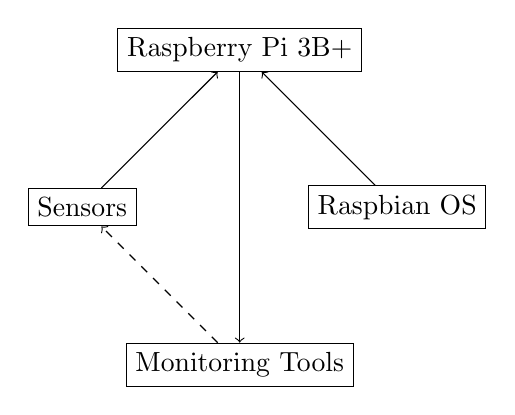
\begin{tikzpicture}
    \node[draw, rectangle] (pi) at (0,0) {Raspberry Pi 3B+};
    \node[draw, rectangle] (sensor) at (-2,-2) {Sensors};
    \node[draw, rectangle] (os) at (2,-2) {Raspbian OS};
    \node[draw, rectangle] (tools) at (0,-4) {Monitoring Tools};

    \draw[->] (sensor) -- (pi);
    \draw[->] (os) -- (pi);
    \draw[->] (pi) -- (tools);

    \draw[->, dashed] (tools) -- (sensor);
\end{tikzpicture}
\caption{Basic System Architecture}
\label{fig:sys_arch}
\end{figure}

\subsection{Simulation Tools and Workload Generation}
\textbf{Computational and Sensor Workloads}:
\begin{itemize}
    \item Implementation of a mixed workload environment, combining both sensor data processing and computationally intensive tasks to evaluate CPU governor performance under varied conditions.
    \item \textit{Sensor Data Handling}: Custom Python scripts to simulate continuous sensor data reading and processing, mimicking typical IoT workloads.
\end{itemize}

\textbf{Computational Tasks}:
\begin{itemize}
    \item \textit{Video Playback}: Use of VLC Media Player for video-based tasks, providing a consistent and measurable workload for CPU performance evaluation.
    \item \textit{Algorithmic Computation}: Implementation of Dijkstra’s algorithm and matrix multiplication in Python to create CPU-intensive tasks, representing complex computational requirements.
\end{itemize}

\subsection{System Monitoring and Performance Metrics}
\textbf{Real-Time Monitoring Tools}:
\begin{itemize}
    \item \textit{psutil Library}: Utilized for real-time monitoring of system metrics, particularly CPU load, to assess the impact of governor changes.
    \item \textit{Custom Python Scripts}: Developed to accurately measure and log system latency and average CPU frequency, capturing the nuanced performance differences under each governor.
\end{itemize}

\textbf{Data Collection and Analysis}:
\begin{itemize}
    \item Performance data is collected and stored in a structured format for subsequent analysis.
    \item Python-based tools (including NumPy and Pandas) are employed for statistical analysis and visualization of the collected data, facilitating a detailed evaluation of each governor's performance.
\end{itemize}

\section{Evaluation}
%This is where you should include your test plan as well as the results of your tests. Clearly identify the metrics considered in the evaluation.. Make sure that you specify all unit tests, integration tests, and “real” tests. The real tests are where you actually schedule tasks using the algorithm in its real-world instance. This way, you can determine if your algorithm actually helped to solve the problem.

%Make sure that you specify your test setup (i.e. how many computers did you use, which were laptops, how many Windows systems, how many Linux systems, what RTOS did you use, what types of embedded systems did you work on, what protocols were involved in your setup, how were your devices connected, who spoke to what at what time and for what reason). You should also specify your procedure very carefully. We should be able to take your equipment and reproduce your tests exactly using the steps that you provide. Please do not miss any details here. Most of this should already be present in your Design Document.

%You should clearly state the “performance metrics” used for the evaluation and also interpret your results. We need to see relevant schedules, plots, charts, and graphs as well as clear interpretations of your data.
\subsection{Testing Methodology}
\textbf{Test Setup and Types}:
\begin{itemize}
    \item \textit{Hardware Setup}: Raspberry Pi 3B+ integrated with DHT11, digital sound sensor, and PIR motion sensor.
    \item \textit{Software Environment}: Raspbian OS with Python for scripting, `psutil` for system monitoring, and Linux tools for governor control.
\end{itemize}

\textbf{Unit Tests}:
\begin{itemize}
    \item \textit{Sensor Scripts}: Validated the accuracy and reliability of sensor data collection scripts.
    \item \textit{Monitoring Scripts}: Tested the functionality of scripts used for recording CPU load, frequency, and latency.
\end{itemize}

\textbf{Integration Tests}:
\begin{itemize}
    \item \textit{System Integration}: Ensured seamless operation between the Raspberry Pi, sensors, and software components.
    \item \textit{Governor Switching}: Verified the effective switching of CPU governors and the corresponding system response.
\end{itemize}

\textbf{Real Tests}:
\begin{itemize}
    \item Executed a series of real-world task scenarios under each governor setting, encompassing both sensor processing and computational tasks.
    \item Recorded performance metrics for each scenario to evaluate the impact of governor choice on system behavior.
\end{itemize}

\subsection{Detailed Procedure for Reproducibility}
\begin{figure}[ht]
    \centering
    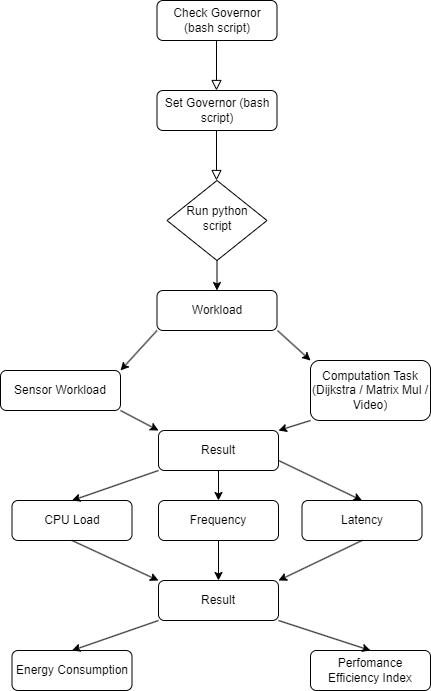
\includegraphics[width=0.75\linewidth]{State Machine.png}
    \caption{Energy Consumption across Different Governors.}
    \label{fig:state_machine}
\end{figure}

\textbf{Hardware Configuration}:
\begin{enumerate}
    \item Connect the DHT11, sound, and PIR sensors to the Raspberry Pi GPIO pins.
    \item Ensure stable power supply and internet connectivity for software updates and monitoring.
\end{enumerate}

\textbf{Software Setup}:
\begin{enumerate}
    \item Install Raspbian OS on the Raspberry Pi.
    \item Set up Python environment, install `psutil`, and other required libraries.
    \item Deploy sensor data collection and performance monitoring scripts.
    \item Configure Linux CPU governor control tools.
\end{enumerate}

\textbf{Execution of Tests}:
\begin{enumerate}
    \item Initiate sensor data collection scripts to simulate continuous data processing.
    \item Run computational tasks (e.g., video playback, Dijkstra's algorithm).
    \item Sequentially switch between different CPU governors, maintaining consistent test conditions.
    \item Collect and log data for CPU load, frequency, latency, and calculate PEI and energy consumption post-test.
\end{enumerate}

\textbf{Data Analysis}:
\begin{enumerate}
    \item Use Python scripts to aggregate and analyze the collected data.
    \item Apply statistical methods to interpret the performance metrics and their implications on CPU governor efficiency.
\end{enumerate}
\subsection{Data Visualization and Analysis}
\subsubsection{CPU Load and Average Frequency across Different Governors}
\begin{figure}[ht]
    \centering
    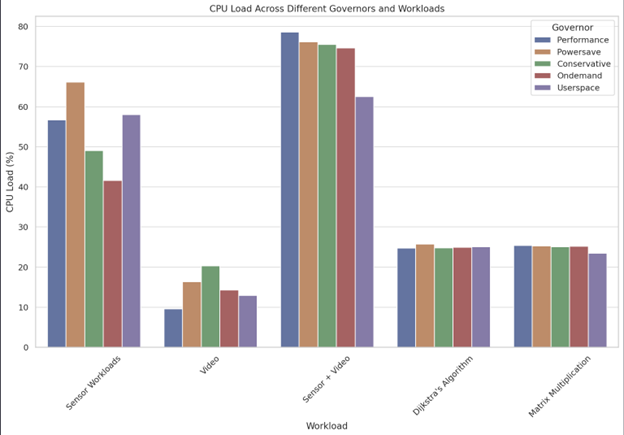
\includegraphics[width=0.75\linewidth]{cpu_load_freq_plot.png}
    \caption{CPU Load across Different Governors.}
    \label{fig:cpu_load_freq}
\end{figure}
\vspace{10pt}
Based on the data, we observe significant variations in CPU load among the different governors and workloads. The `Powersave` governor exhibits the highest average CPU load at 66.13\% for sensor workloads, while for more intensive tasks like matrix multiplication, it maintains a CPU load of 25.28\%. This suggests that while the `Powersave` governor reduces frequency to 600 MHz to conserve energy, it results in higher CPU utilization, which could lead to longer task completion times.

The `Performance` governor, with a consistent frequency of 1400 MHz, showcases an interesting pattern: it has a relatively high CPU load for sensor workloads at 56.66\%, yet it handles intensive computational tasks like Dijkstra's algorithm with a lower CPU load of 24.74\%. This governor optimizes for speed and appears to be more efficient when the system is under a heavy computational workload.

Adaptive governors, `Ondemand` and `Conservative`, show their ability to balance load and performance. Under sensor workloads, `Ondemand` lowers the CPU load to 41.63\% with an average frequency of 1397 MHz, suggesting a more aggressive response to load changes. `Conservative` has a similar load of 49.07\% but maintains the maximum frequency of 1400 MHz, indicating that it may not downscale the frequency as efficiently during lighter tasks.

`Userspace`, with manual frequency settings, shows a load of 58.03\% for sensor workloads at 1400 MHz, and interestingly, a load of 12.95\% for video playback at 800 MHz, which illustrates the impact of tailored frequency settings on CPU load management. 

\subsubsection{Latency across Different Governors and Workloads}
\begin{figure}[ht]
    \centering
    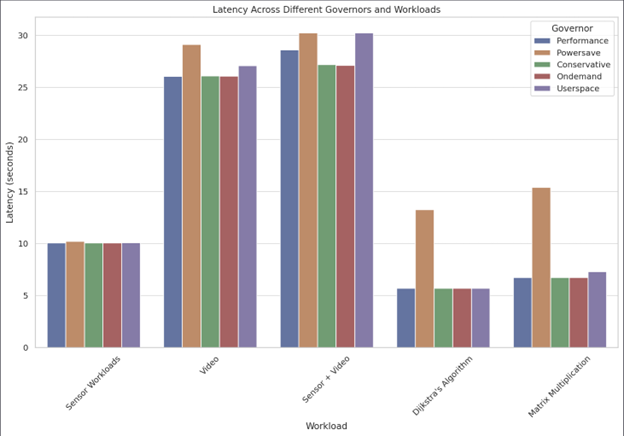
\includegraphics[width=0.75\linewidth]{cpu_latency_plot.png}
    \caption{Latency across Different Governors and Workloads.}
    \label{fig:latency}
\end{figure}
\vspace{10pt}

The latency characteristics for each governor across diverse workloads reveal critical insights into their performance. The `Performance` governor demonstrates consistently low latency across all tasks, with an exemplary mean latency of 10.054 seconds for sensor workloads and only a slight increase to 26.071 ms for video playback. These values underscore the governor's design to prioritize swift task execution.

Conversely, the `Powersave` governor shows significantly higher latency, particularly notable in computationally intensive tasks such as Dijkstra's algorithm and matrix multiplication, with mean latencies of 13.2523 second and 15.3913 seconds, respectively. This indicates a considerable performance compromise for energy savings, as the reduced frequency leads to longer task completion times.

Adaptive governors like `Ondemand` and `Conservative` offer an interesting balance, with `Ondemand` slightly outperforming `Conservative` in most tasks. For example, under `Ondemand`, the latency for sensor workloads is a mean of 10.046 seconds, marginally lower than `Conservative`'s 10.0633 seconds, suggesting a more efficient frequency scaling in response to workload demands.

The `Userspace` governor, which is subject to manual frequency control, shows latencies that are competitive with the `Performance` governor for lighter workloads but exhibit a notable increase to 27.100 ms for video tasks when set to sub-optimal frequencies.

\subsubsection{Energy Consumption across Different Governors}
\begin{figure}[ht]
    \centering
    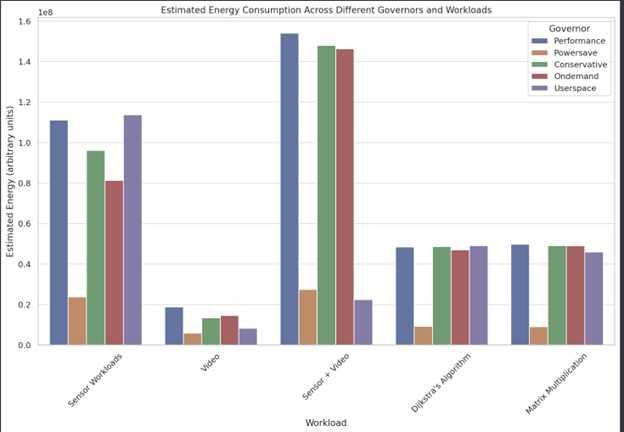
\includegraphics[width=0.75\linewidth]{energy_consumption_plot.png}
    \caption{Energy Consumption across Different Governors.}
    \label{fig:energy_consumption}
\end{figure}
\vspace{10pt}
The estimated energy consumption, as illustrated in the plot, varies notably among the CPU governors and workloads. For instance, the `Performance` governor, which operates at the maximum frequency of 1400 MHz, exhibits the highest energy consumption across all workloads. Specifically, for sensor workload + video playback, it reaches approximately \(1.54 \times 10^8\) energy units, reflecting its design priority for maximum throughput at the cost of power efficiency.

On the other end of the spectrum, the `Powersave` governor significantly reduces energy consumption, with sensor workloads consuming as low as \(2.38 \times 10^7\) energy units. However, for computationally intensive tasks such as Dijkstra's algorithm, it shows an increase up to \(9.26 \times 10^7\) energy units, which is still considerably less than what's observed under the `Performance` governor.

The `Ondemand` governor demonstrates adaptive energy consumption, dynamically adjusting based on the workload. For example, the energy consumption for sensor workloads is around \(8.12 \times 10^7\) energy units, positioning itself as an intermediate between the `Performance` and `Powersave` governors.

The `Conservative` governor showcases similar adaptability but tends to consume slightly more energy than `Ondemand`, indicative of its cautious approach to increasing frequency. For instance, in matrix multiplication tasks, it consumes roughly \(4.92 \times 10^7\) energy units, marginally higher compared to `Ondemand`.

The `Userspace` governor, with customizable settings, shows varied energy consumption patterns, largely dependent on the specific frequencies set by the user. Its energy consumption for video playback tasks is about \(8.29 \times 10^7\) energy units, which suggests a middle ground approach, not fully optimized for power saving nor performance.

\subsubsection{Performance Efficiency Index (PEI) across Different Governors}
\begin{figure}[ht]
    \centering
    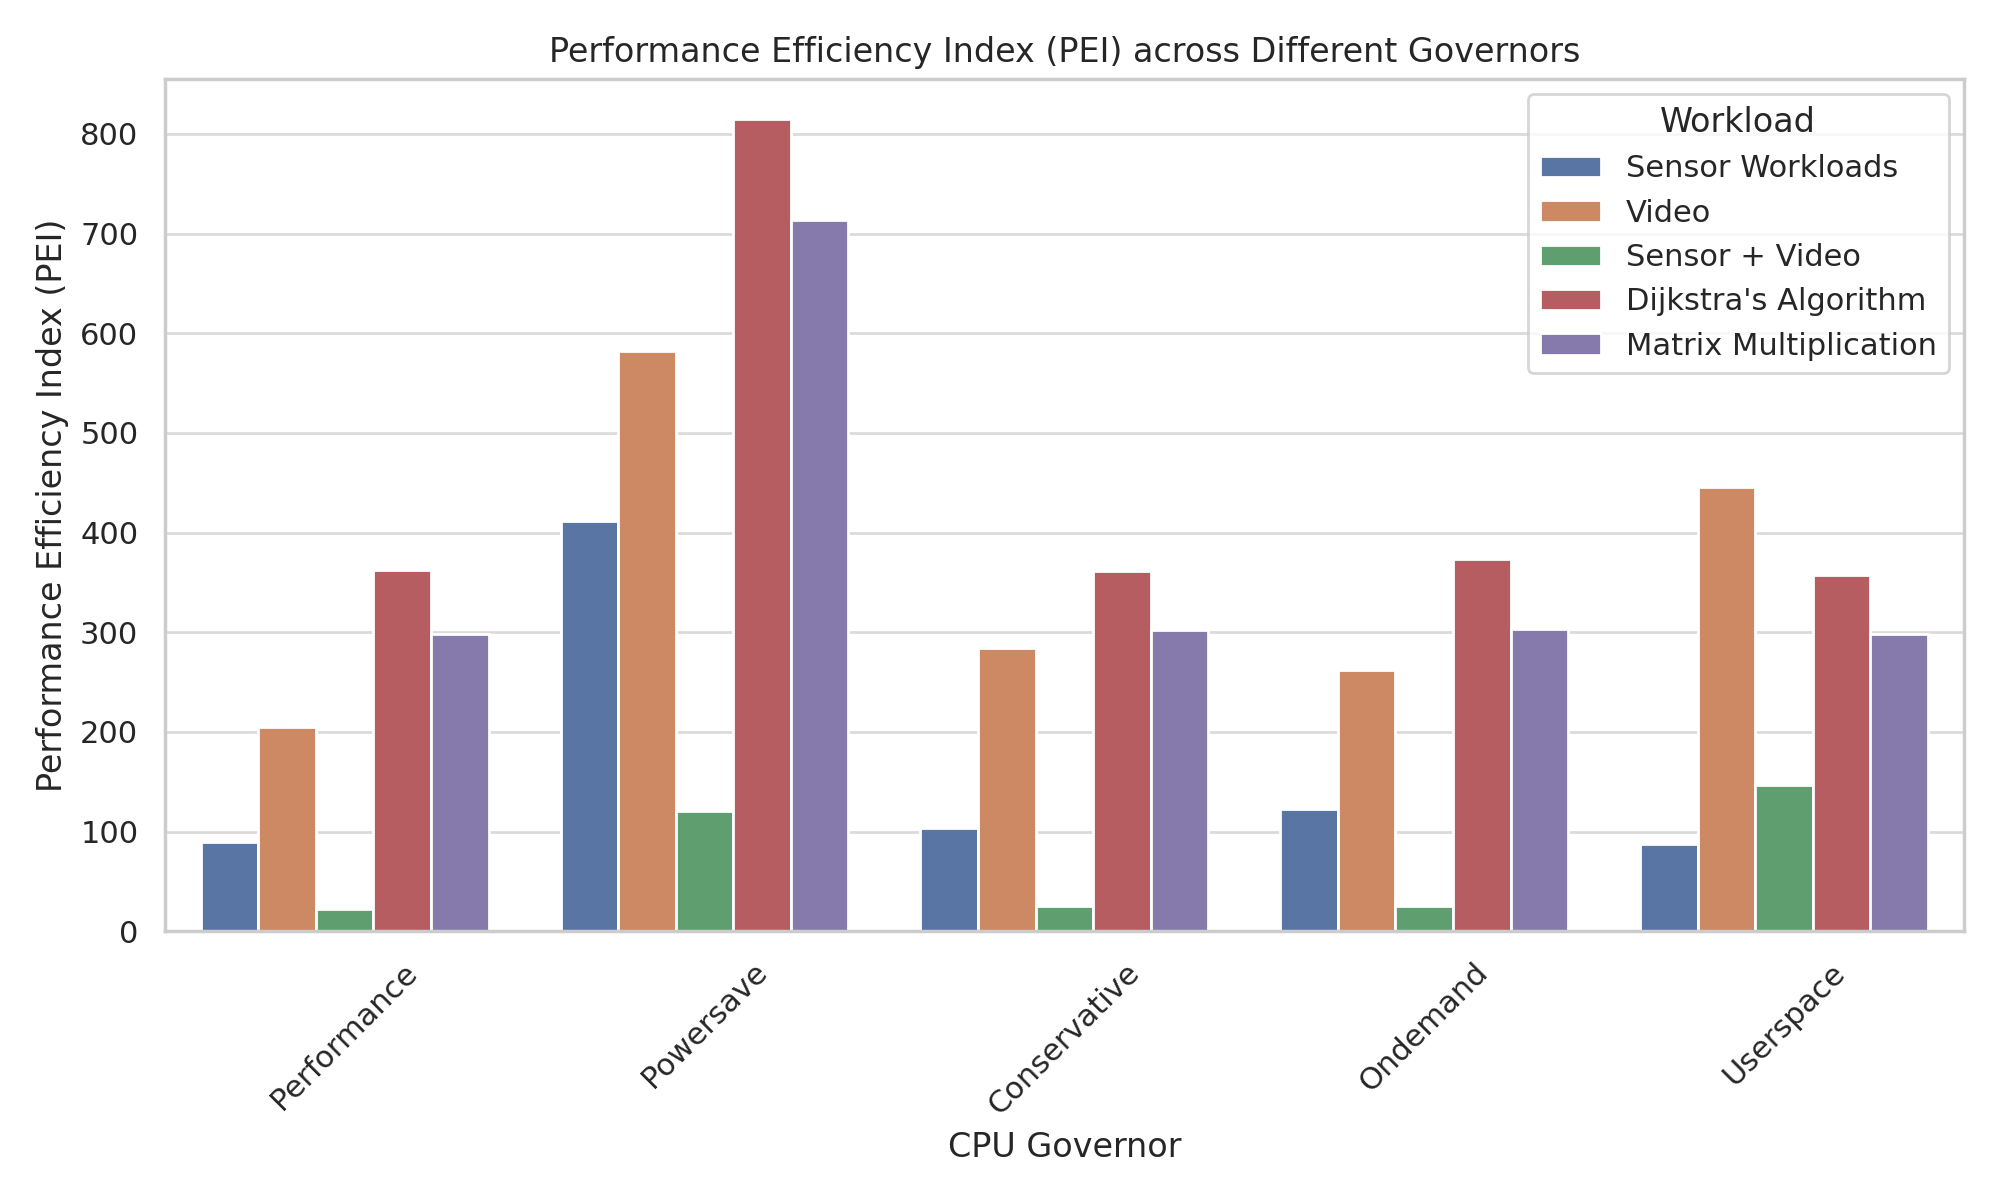
\includegraphics[width=0.9\linewidth]{pei_plot.png}
    \caption{Performance Efficiency Index (PEI) across Different Governors.}
    \label{fig:pei}
\end{figure}
\vspace{10pt}
The PEI plot demonstrates a varied efficiency landscape across the spectrum of governors. The `Performance` governor, designed for speed, shows lower PEI values across computationally intensive tasks such as Dijkstra's Algorithm and Matrix Multiplication. This is indicative of the trade-off between quick task execution and energy consumption.

On the other end, the `Powersave` governor exhibits higher PEI values, especially in less demanding workloads like Sensor Workloads, suggesting that tasks can be completed with substantially lower energy consumption, albeit potentially at slower speeds. This aligns with the governor's goal to conserve energy, which may suit applications where time efficiency is less critical.

The `Ondemand` governor displays intermediate PEI values, reflecting its dynamic adjustment to CPU load and latency. For workloads that are sporadic or unpredictable, such as Sensor + Video, `Ondemand` offers a balance between responsiveness and energy use, optimizing performance as workload demands increase.

The `Conservative` governor typically trails the `Ondemand` in terms of PEI, suggesting a slightly less efficient response to workload changes. Its cautious frequency scaling can lead to increased task completion times, which might not be ideal for time-sensitive applications but could benefit scenarios where gradual changes in demand are expected.

Lastly, the `Userspace` governor showcases the impact of user-defined settings, with PEI values varying widely depending on how the frequency is managed for each task. When optimally configured, `Userspace` can achieve high performance efficiency, as seen in the Sensor Workloads.

\section{Conclusions}

This study involves a comprehensive analysis of the effects of various CPU governors on the performance and energy consumption of a Raspberry Pi 3B+ under different workload conditions. The experiment leveraged the inherent capabilities of Dynamic Voltage and Frequency Scaling (DVFS) to adjust the CPU's operational parameters, aiming to discover an optimal balance between performance efficiency and power consumption.

Our contributions to this field of research include:
\begin{itemize}
    \item A dataset capturing CPU Load, Average Frequency, and Latency across five distinct CPU governors under various workloads.
    \item A novel estimation of energy consumption and Performance Efficiency Index (PEI) that takes into account both the operational frequency and the CPU load.
    \item A systematic comparison of the governors' performance, providing a nuanced understanding of their behavior in real-time systems.
\end{itemize}

Findings from the experiment indicate that:
\begin{itemize}
    \item The `Performance` governor, while ensuring the lowest latency, resulted in the highest energy consumption across all workloads.
    \item The `Powersave` governor significantly improved energy efficiency but at the expense of increased latency, which may not be suitable for time-sensitive tasks.
    \item Adaptive governors (`Ondemand` and `Conservative`) offered a middle ground, dynamically scaling frequency based on workload demands, hence providing a balanced approach.
    \item The `Userspace` governor, with manual frequency settings, allowed for tailored performance tuning, indicating its potential for workload-specific optimization.
\end{itemize}

From these findings, we recommend:
\begin{itemize}
    \item Further empirical studies to determine the exact power characteristics of CPU governors, which would enable more accurate energy consumption models.
    \item Development of advanced governor algorithms that can learn from workload patterns and predictively adjust frequencies for improved efficiency.
    \item Exploration of the impact of different governors in multi-core environments, as well as their effects on the thermal performance of the system.
\end{itemize}

Future experiments could focus on the integration of machine learning techniques to create smart governors that dynamically adapt to the system's workload patterns, potentially enhancing energy efficiency without compromising on performance. Additionally, considering the evolving landscape of IoT devices, further research could also explore the governors' behavior in a wider array of hardware configurations and operational environments.


\section{References}
\nocite{*}  
\printbibliography[heading=none]
\section{Appendix}
\subsection{Self-Assessment of Project Completion}
\begin{figure}[ht]
    \centering
    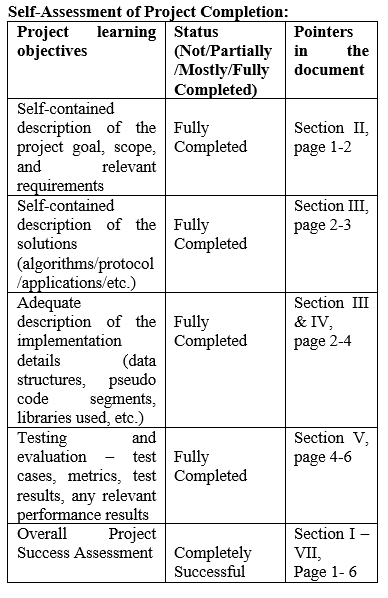
\includegraphics[width=0.75\linewidth]{self_reflection.png}
    \caption{Self-Assessment of Project}
    \label{fig:self_assess}
\end{figure}

\subsection{Team Member Contributions}
\begin{figure}[ht]
    \centering
    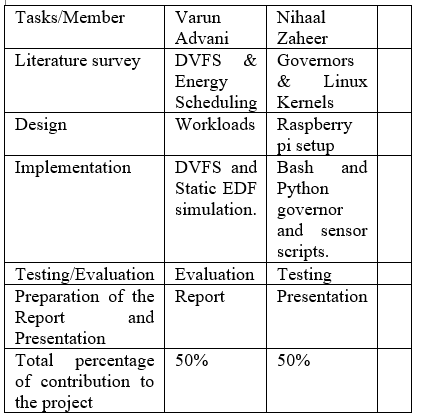
\includegraphics[width=0.75\linewidth]{team_member_contrib.png}
    \caption{Team Member Contribution}
    \label{fig:contrib}
\end{figure}

\end{document}
